\documentclass[11pt]{article}

\usepackage[a4paper,margin=1in]{geometry}
\usepackage[T1]{fontenc}
\usepackage[utf8]{inputenc}
\usepackage{lmodern}
\usepackage{microtype}
\usepackage{amsmath}
\usepackage{amssymb}
\usepackage{booktabs}
\usepackage{multirow}
\usepackage{graphicx}
\usepackage{subcaption}
\usepackage{float}
\usepackage{siunitx}
\usepackage{hyperref}
\usepackage{xcolor}
\usepackage{enumitem}

\hypersetup{
    colorlinks=true,
    linkcolor=blue!60!black,
    citecolor=blue!60!black,
    urlcolor=blue!60!black
}

\sisetup{
    round-mode=places,
    round-precision=3,
    table-number-alignment=center
}

\title{Does Compression Forget Cancer?\\
\large Efficient Medical Vision Transformers for Edge Dermatology: Pruning, Quantization, and Distillation with Diagnostic Safety Analysis}

\author{
[Student Name] \and [Teammate Name] \\
\small TinyML / Efficient Deep Learning Final Project
}

\date{\today}

\begin{document}

\maketitle

\begin{abstract}
Deploying skin-lesion classifiers on edge devices requires aggressive model compression, but standard compression metrics can obscure clinically dangerous failures on rare and high-risk classes such as melanoma. In this project, we study whether compressing medical Vision Transformers causes them to forget dangerous diseases before benign classes. We fine-tune DeiT-Tiny and DeiT-Small on the HAM10000 dermoscopy dataset and compare four one-shot pruning criteria: magnitude, Wanda, Taylor, and random pruning. We then evaluate three additional compression questions: whether sensitivity-guided non-uniform sparsity allocation is safer than uniform pruning, whether post-training INT8 quantization stacks safely on top of pruning, and whether knowledge distillation improves pruning robustness. Our evaluation emphasizes balanced accuracy and per-class sensitivity, especially melanoma recall. On the dense baseline, DeiT-Small achieved balanced accuracy $0.862$ and melanoma sensitivity $0.753$, while DeiT-Tiny achieved balanced accuracy $0.840$ and melanoma sensitivity $0.758$. At $50\%$ sparsity, magnitude pruning preserved overall diagnostic performance better than Wanda on both models. For DeiT-Small, magnitude retained balanced accuracy $0.813$ and melanoma sensitivity $0.637$, whereas Wanda fell to balanced accuracy $0.685$ and melanoma sensitivity $0.444$. Taylor pruning was highly competitive and achieved the strongest melanoma sensitivity at $50\%$ sparsity on DeiT-Small ($0.677$), though magnitude yielded the best balanced accuracy. Sensitivity-guided non-uniform pruning strongly improved Wanda, increasing DeiT-Small from balanced accuracy $0.685$ to $0.811$ and melanoma sensitivity from $0.444$ to $0.632$ at the same average sparsity. INT8 quantization was nearly lossless on the dense model and only mildly degraded magnitude-pruned models while reducing size and CPU latency. Distillation improved the unpruned Tiny baseline but did not improve pruning robustness. Overall, our results show that activation-aware Wanda did not protect melanoma sensitivity better than simpler pruning criteria in this medical vision setting, while non-uniform allocation was the most effective strategy for recovering safety under a weak pruning policy.
\end{abstract}

\section{Introduction}
Edge deployment of medical AI systems is an important practical goal. In dermatology, portable or clinic-side devices could support screening in low-connectivity settings, reduce latency, and improve privacy by avoiding cloud inference. However, these advantages require compact models that can run efficiently under hardware and memory constraints. Compression therefore becomes essential.

In medical classification, compression quality cannot be judged only by overall accuracy. HAM10000 is strongly imbalanced, with melanocytic nevi dominating the dataset while high-risk classes such as melanoma appear much less frequently. A compressed model can preserve aggregate accuracy while becoming worse at detecting exactly the diseases clinicians care most about. This makes class-wise sensitivity, particularly melanoma sensitivity, a much more meaningful safety-oriented evaluation target than top-line accuracy alone.

This project asks the following question: when a medical Vision Transformer is compressed, does it forget dangerous diseases first? To answer that, we compare multiple pruning criteria on two DeiT models trained on HAM10000 and evaluate them with clinical metrics. We then extend the study in three directions. First, we test whether layer sensitivity can guide a safer non-uniform sparsity allocation. Second, we examine whether INT8 quantization stacks safely on top of pruning. Third, we test whether knowledge distillation produces features that are more robust to pruning.

Our findings are both practical and surprising. In this setup, activation-aware Wanda does not preserve clinical safety better than magnitude pruning, and Taylor pruning is often competitive or better for melanoma sensitivity. At the same time, sensitivity-guided non-uniform pruning substantially improves Wanda and nearly closes the gap to the stronger criteria. These results suggest that in medical vision, where a model is pruned may matter more than the nominal sophistication of the score function itself.

\section{Related Work}
The HAM10000 dataset introduced a diverse benchmark for automated dermoscopic lesion analysis and made class-imbalanced skin-lesion classification widely accessible to academic machine learning research~\cite{tschandl2018ham10000}. For transformer-based image classification, DeiT demonstrated that Vision Transformers can be trained efficiently on ImageNet-scale data without massive external pretraining, making them a practical backbone choice for transfer learning and domain adaptation~\cite{touvron2021deit}.

Model pruning has a long history in neural network compression. Magnitude pruning remains a strong baseline due to its simplicity and surprising robustness. First-order Taylor-based pruning approximates the effect of removing parameters through gradients and has been shown to outperform naive criteria in transfer-learning settings~\cite{molchanov2017taylor}. More recently, Wanda proposed a simple activation-aware score for pruning pretrained large language models by combining weight magnitude and input activation statistics~\cite{sun2023wanda}. Although Wanda was designed for LLMs, its activation-aware formulation makes it interesting to test in medical Vision Transformers, where token-like patch representations may also contain outlier information.

Quantization and distillation are also standard ingredients of deployment pipelines. Integer quantization provides strong reductions in storage and latency with modest accuracy loss when applied carefully~\cite{jacob2018quantization}. Knowledge distillation transfers a teacher model's predictive structure to a smaller student and often improves the smaller model's dense accuracy~\cite{hinton2015distillation}. What remains less understood is how these methods interact with pruning under medically meaningful class-wise safety constraints.

\section{Methodology}
\subsection{Dataset}
We use HAM10000, a publicly available dermoscopic dataset containing 10{,}015 images across seven diagnostic classes: actinic keratosis/intraepithelial carcinoma (\texttt{akiec}), basal cell carcinoma (\texttt{bcc}), benign keratosis-like lesions (\texttt{bkl}), dermatofibroma (\texttt{df}), melanoma (\texttt{mel}), melanocytic nevus (\texttt{nv}), and vascular lesions (\texttt{vasc})~\cite{tschandl2018ham10000}. The dataset is strongly imbalanced, with nevi forming the majority class. We use a stratified 80/20 train-validation split and weighted cross-entropy during training.

\subsection{Models}
We fine-tune two transformer backbones from \texttt{timm}: DeiT-Tiny and DeiT-Small~\cite{touvron2021deit}. In both cases, the ImageNet head is replaced with a seven-class classification head. DeiT-Tiny serves as the smaller edge-oriented student-like model, while DeiT-Small provides a stronger accuracy baseline and later serves as the teacher in the distillation experiments.

\subsection{Fine-Tuning}
Both models are fine-tuned using AdamW with a learning rate of $10^{-4}$, weight decay $0.05$, cosine scheduling, and standard augmentation including random crop, flips, and color jitter. Weighted cross-entropy is used to reduce the effect of class imbalance. Balanced accuracy on the validation set is used as the checkpoint-selection criterion.

\subsection{Pruning Criteria}
We compare four one-shot unstructured pruning criteria:
\begin{itemize}[leftmargin=1.2em]
    \item \textbf{Magnitude}: keep weights with largest absolute value.
    \item \textbf{Wanda}: score each weight by $|w| \cdot \|x\|$, where $\|x\|$ is the input activation norm for the corresponding feature~\cite{sun2023wanda}.
    \item \textbf{Taylor}: score each weight by $|w \cdot \frac{\partial \mathcal{L}}{\partial w}|$, following first-order Taylor reasoning~\cite{molchanov2017taylor}.
    \item \textbf{Random}: random scores as a lower-bound control.
\end{itemize}

Pruning is applied globally across eligible linear layers at sparsity levels of 20\%, 40\%, 50\%, 60\%, and 70\%. The classifier head, class token, positional embedding, and patch embedding projection are excluded from pruning in the main setup because these small components can disproportionately destabilize performance. Each experiment reloads the dense checkpoint before masks are applied.

\subsection{Non-Uniform Sparsity Allocation}
To test whether uniform sparsity is unnecessarily harmful, we estimate per-layer sensitivity by pruning one layer at a time and measuring balanced accuracy drop. Layers are then ranked and assigned lower or higher sparsity according to their sensitivity while keeping the overall average sparsity fixed at 50\%. We evaluate this policy for both magnitude and Wanda.

\subsection{Quantization}
We apply dynamic INT8 quantization on CPU to the dense model and to the best 50\% pruned configurations. This allows us to test whether quantization is a safe late-stage compression step and to measure model size and latency trade-offs.

\subsection{Knowledge Distillation}
We distill DeiT-Small into DeiT-Tiny using a standard soft-target distillation loss with temperature $T=4$ and mixing coefficient $\alpha=0.7$~\cite{hinton2015distillation}. We then compare three Tiny variants: directly fine-tuned, distilled, and ImageNet-only pretrained. Each is evaluated both before and after Wanda pruning at 50\% sparsity.

\section{Experimental Setup}
All experiments were run locally on an NVIDIA RTX 3060 Ti after the planned MBZUAI cluster workflow became unavailable. This affected throughput and batch size but did not prevent the full experiment set from being completed. The final implementation generated checkpoints, pruning masks, log CSVs, and report figures in PDF format.

We report:
\begin{itemize}[leftmargin=1.2em]
    \item overall accuracy,
    \item balanced accuracy,
    \item per-class sensitivity,
    \item melanoma sensitivity as the primary safety metric,
    \item model size in KB,
    \item CPU inference latency in milliseconds.
\end{itemize}

\section{Results}

\subsection{Dense Baselines}
The dense baselines are shown in Table~\ref{tab:baseline}. DeiT-Small provides the strongest aggregate performance with balanced accuracy $0.862$, while DeiT-Tiny remains competitive at $0.840$. Melanoma sensitivity is very similar between the two models, with Tiny slightly higher in this run. DeiT-Small also provides much stronger recall on dermatofibroma and benign keratosis.

\begin{table}[H]
    \centering
    \caption{Dense baseline performance on HAM10000.}
    \label{tab:baseline}
    \begin{tabular}{lSSSS}
        \toprule
        Model & {Overall Acc.} & {Balanced Acc.} & {Mel. Sens.} & {BCC Sens.} \\
        \midrule
        DeiT-Tiny  & 0.849 & 0.840 & 0.758 & 0.913 \\
        DeiT-Small & 0.889 & 0.862 & 0.753 & 0.903 \\
        \bottomrule
    \end{tabular}
\end{table}

\subsection{Pruning Criterion Comparison}
Figure~\ref{fig:melanoma} and Figure~\ref{fig:balanced} show the main pruning trends. Random pruning collapses quickly, as expected. More importantly, Wanda does not outperform magnitude pruning in this medical ViT setting. At 50\% sparsity, magnitude pruning is consistently safer than Wanda on both models, while Taylor pruning is highly competitive and preserves melanoma sensitivity especially well on DeiT-Small.

\begin{table}[H]
    \centering
    \caption{Comparison at 50\% sparsity.}
    \label{tab:sparsity50}
    \begin{tabular}{llSSS}
        \toprule
        Model & Criterion & {Balanced Acc.} & {Mel. Sens.} & {Size (KB)} \\
        \midrule
        \multirow{4}{*}{DeiT-Tiny}
            & Magnitude & 0.804 & 0.677 & 11217.0 \\
            & Wanda     & 0.614 & 0.556 & 11217.0 \\
            & Taylor    & 0.720 & 0.538 & 11217.0 \\
            & Random    & 0.177 & 0.000 & 11217.0 \\
        \midrule
        \multirow{4}{*}{DeiT-Small}
            & Magnitude & 0.813 & 0.637 & 43170.0 \\
            & Wanda     & 0.685 & 0.444 & 43170.0 \\
            & Taylor    & 0.801 & 0.677 & 43170.0 \\
            & Random    & 0.143 & 0.000 & 43170.0 \\
        \bottomrule
    \end{tabular}
\end{table}

For DeiT-Tiny, magnitude pruning remains strong through 50\% sparsity and degrades gradually afterward. Wanda degrades much earlier, especially in balanced accuracy. For DeiT-Small, magnitude again provides the strongest balanced accuracy under pruning, while Taylor yields the best melanoma sensitivity at 50\%. This is important for the project hypothesis: the activation-aware criterion did not protect melanoma detection better than simpler baselines.

\begin{figure}[H]
    \centering
    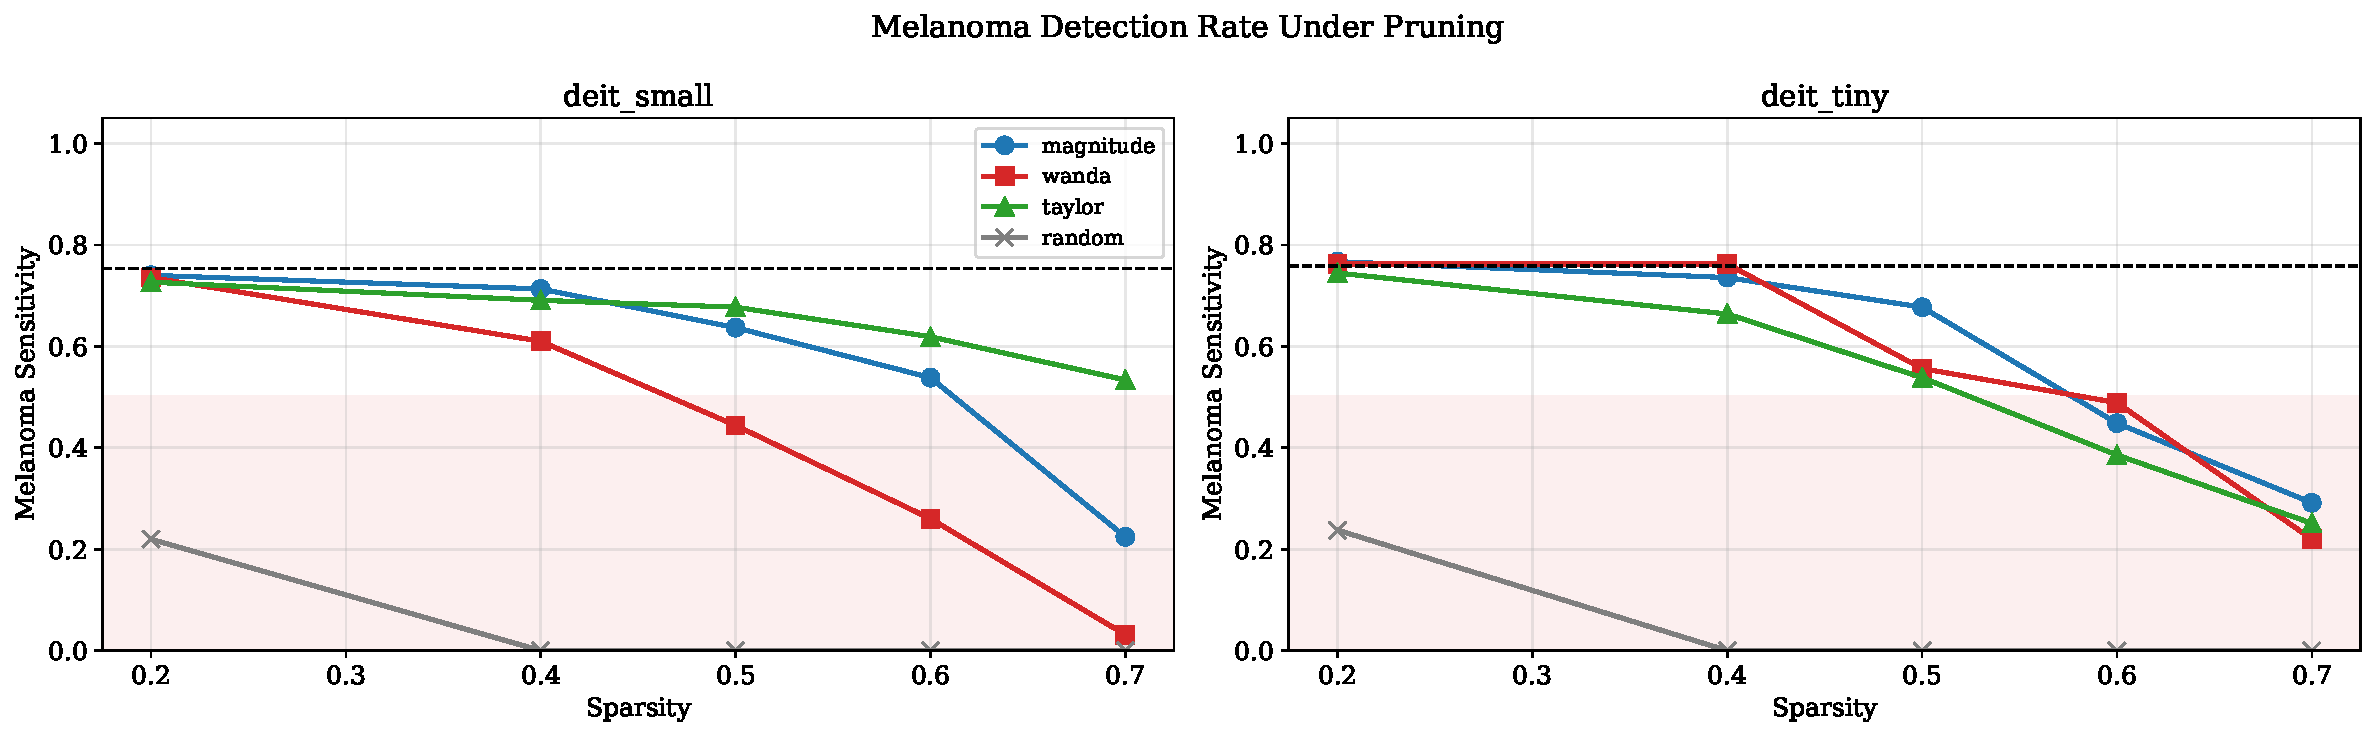
\includegraphics[width=\textwidth]{../results/figures_local/fig1_melanoma_sensitivity.pdf}
    \caption{Melanoma sensitivity under pruning for DeiT-Tiny and DeiT-Small.}
    \label{fig:melanoma}
\end{figure}

\begin{figure}[H]
    \centering
    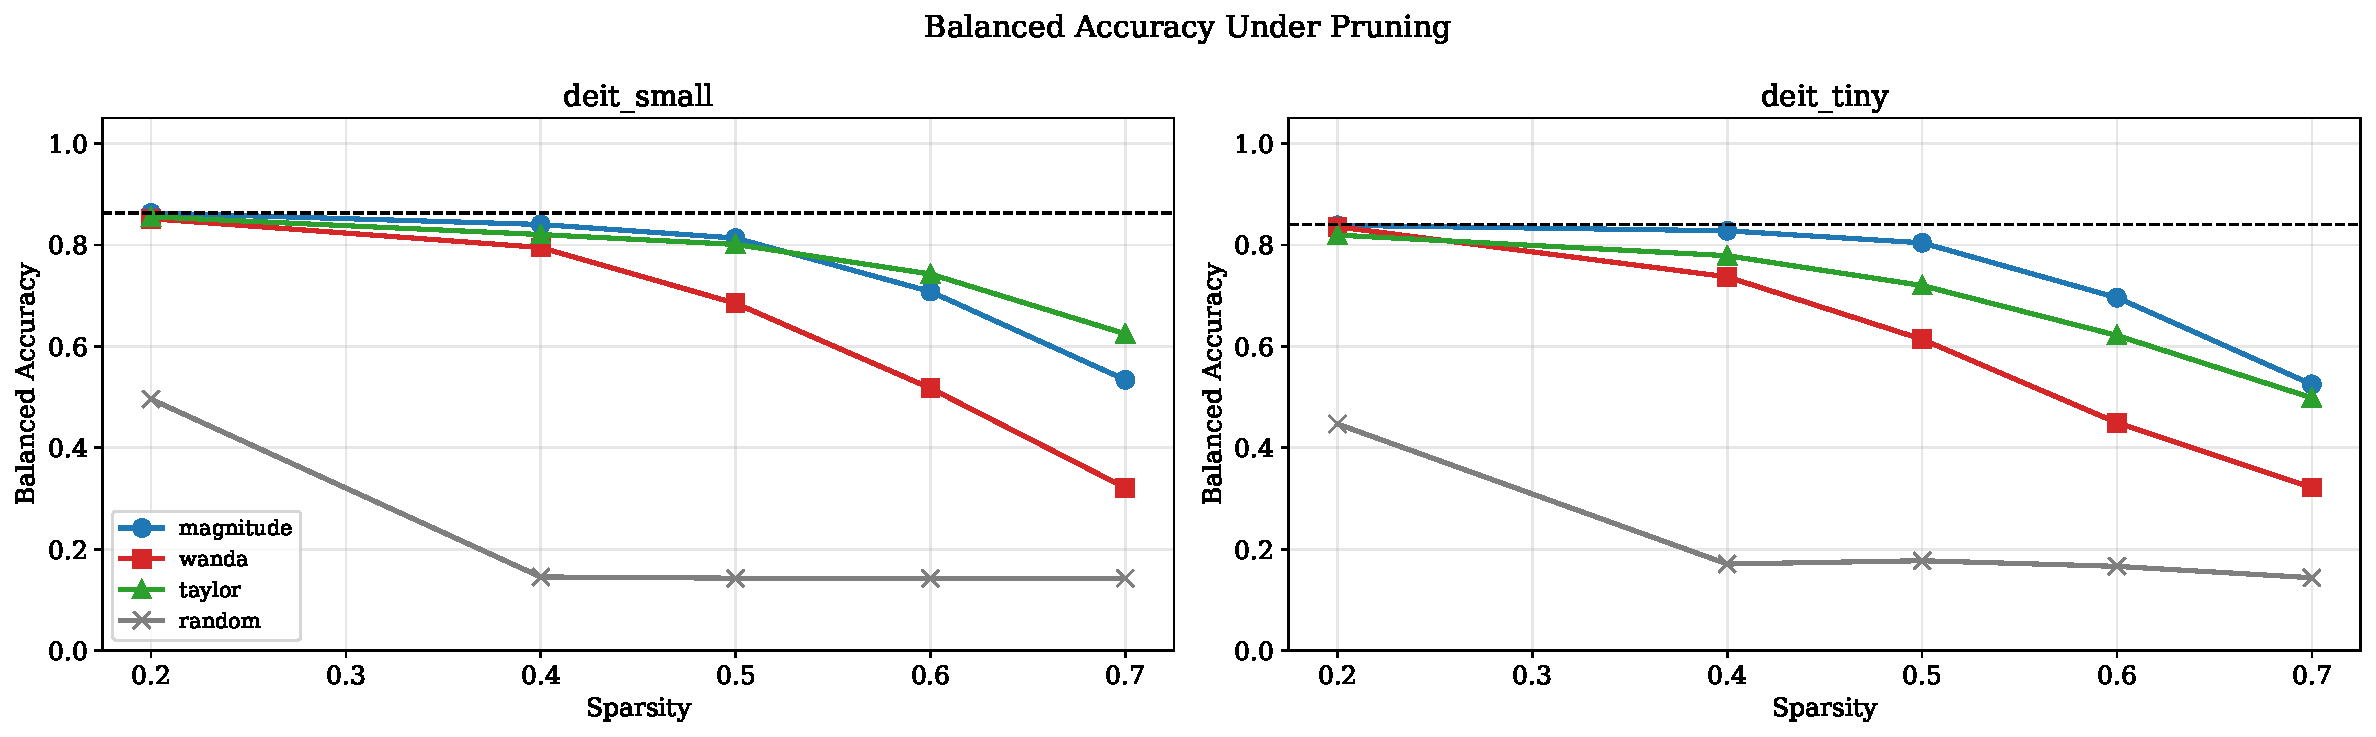
\includegraphics[width=\textwidth]{../results/figures_local/fig2_balanced_accuracy.pdf}
    \caption{Balanced accuracy under pruning for DeiT-Tiny and DeiT-Small.}
    \label{fig:balanced}
\end{figure}

\subsection{Per-Layer-Type Sensitivity}
The per-layer breakdown in Table~\ref{tab:perlayer} and Figure~\ref{fig:perlayer} shows that MLP layers are the most sensitive group, especially for Wanda. Pruning only the MLP at 50\% sparsity with Wanda causes a balanced accuracy drop of about $0.104$, far larger than pruning QKV or attention output layers. Magnitude pruning on the MLP is less harmful but still meaningfully degrades performance. In contrast, pruning QKV or attention output layers has relatively small effect.

Patch embedding should be interpreted cautiously. In our code, patch embedding projection is excluded from default pruning, so the patch embedding rows effectively behave like an unpruned control. The result is still useful because it confirms that the performance drop is driven by the actually pruned groups.

\begin{table}[H]
    \centering
    \caption{Per-layer-type pruning on DeiT-Small at 50\% sparsity. Values are balanced accuracy drops from the dense DeiT-Small baseline.}
    \label{tab:perlayer}
    \begin{tabular}{lSS}
        \toprule
        Layer Type & {Wanda Drop} & {Magnitude Drop} \\
        \midrule
        QKV         & 0.011 & 0.008 \\
        Attention Output & 0.017 & 0.000 \\
        MLP         & 0.104 & 0.022 \\
        Patch Embed & 0.000 & 0.000 \\
        \bottomrule
    \end{tabular}
\end{table}

\begin{figure}[H]
    \centering
    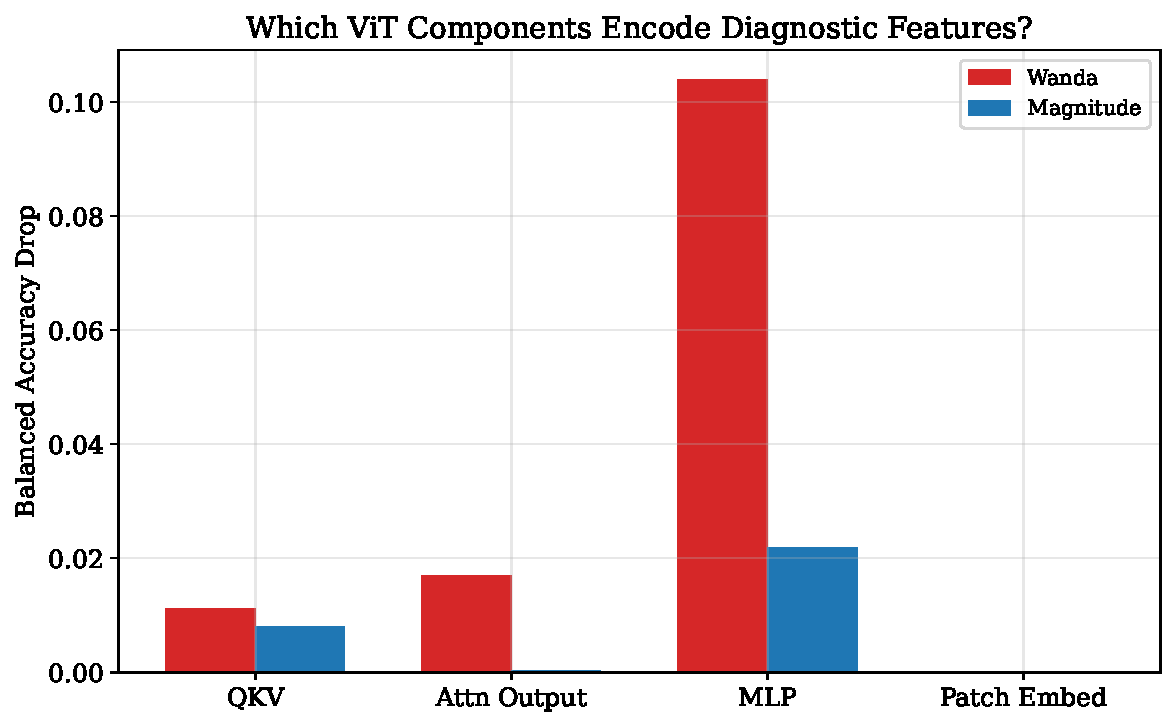
\includegraphics[width=0.9\textwidth]{../results/figures_local/fig3_perlayer_bars.pdf}
    \caption{Balanced accuracy drop when pruning only one ViT component type at 50\% sparsity.}
    \label{fig:perlayer}
\end{figure}

\subsection{Sensitivity-Guided Non-Uniform Allocation}
The non-uniform experiment produced one of the strongest findings in the project. Table~\ref{tab:nonuniform} and Figure~\ref{fig:nonuniform} show that non-uniform allocation is highly beneficial for Wanda. Uniform Wanda at 50\% sparsity yields balanced accuracy $0.685$ and melanoma sensitivity $0.444$, but non-uniform Wanda recovers these to $0.811$ and $0.632$ respectively. This nearly closes the gap to uniform magnitude pruning.

For magnitude pruning, however, non-uniform allocation does not help. The non-uniform magnitude configuration drops from balanced accuracy $0.813$ to $0.784$ while leaving melanoma sensitivity unchanged at $0.637$. This suggests that magnitude pruning is already allocating damage in a fairly robust way under global pruning, whereas Wanda benefits substantially from explicit layer-level protection.

\begin{table}[H]
    \centering
    \caption{Uniform vs. non-uniform pruning at target average sparsity 50\% on DeiT-Small.}
    \label{tab:nonuniform}
    \begin{tabular}{llSS}
        \toprule
        Criterion & Condition & {Balanced Acc.} & {Mel. Sens.} \\
        \midrule
        \multirow{3}{*}{Magnitude}
            & Dense      & 0.862 & 0.753 \\
            & Uniform    & 0.813 & 0.637 \\
            & Non-uniform & 0.784 & 0.637 \\
        \midrule
        \multirow{3}{*}{Wanda}
            & Dense      & 0.862 & 0.753 \\
            & Uniform    & 0.685 & 0.444 \\
            & Non-uniform & 0.811 & 0.632 \\
        \bottomrule
    \end{tabular}
\end{table}

\begin{figure}[H]
    \centering
    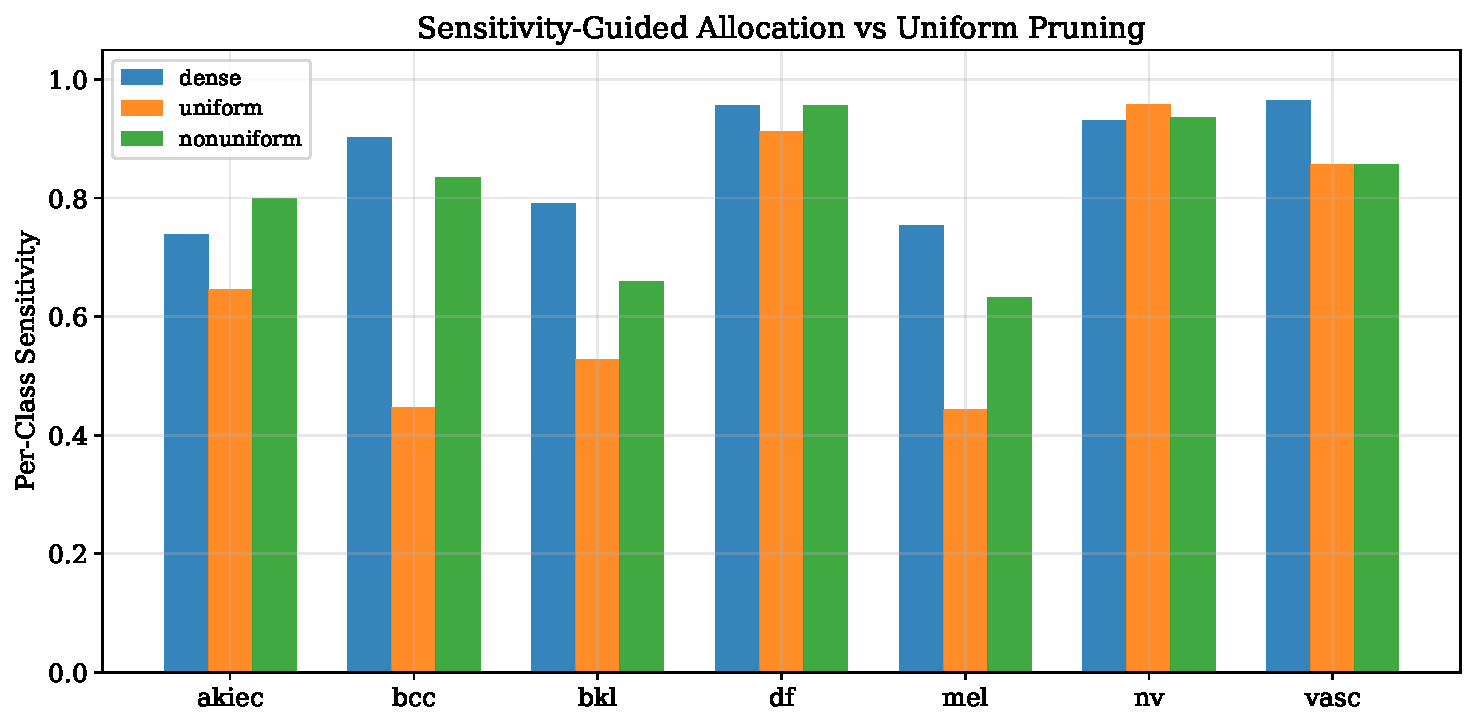
\includegraphics[width=0.95\textwidth]{../results/figures_local/fig4_nonuniform_vs_uniform.pdf}
    \caption{Per-class sensitivity for dense, uniform, and non-uniform pruning. The plotted file corresponds to the Wanda case, where the rescue effect is strongest.}
    \label{fig:nonuniform}
\end{figure}

\subsection{Quantization Stacking}
INT8 quantization is comparatively safe in this project. The dense quantized-only DeiT-Small model reduces size from 84.7 MB to 22.5 MB and improves CPU latency from 22.27 ms to 15.72 ms with negligible loss in balanced accuracy. This already makes quantization a strong deployment tool.

Stacking quantization on top of pruning produces different outcomes depending on pruning quality. For magnitude-pruned DeiT-Small, balanced accuracy decreases only slightly from $0.813$ to $0.804$ and melanoma sensitivity from $0.637$ to $0.632$. For Wanda-pruned DeiT-Small, the additional degradation is also modest relative to the much larger loss already introduced by Wanda pruning. Thus, quantization is not the main safety risk in the pipeline; the pruning choice matters far more.

\begin{table}[H]
    \centering
    \caption{Quantization and pruning stacking on DeiT-Small.}
    \label{tab:quant}
    \begin{tabular}{llSSS}
        \toprule
        Configuration & Criterion & {Balanced Acc.} & {Mel. Sens.} & {Latency (ms)} \\
        \midrule
        Dense & None & 0.862 & 0.753 & 22.27 \\
        Quantized only & None & 0.862 & 0.753 & 15.72 \\
        Pruned only & Wanda & 0.685 & 0.444 & 21.94 \\
        Pruned + Quantized & Wanda & 0.666 & 0.435 & 15.90 \\
        Pruned only & Magnitude & 0.813 & 0.637 & 22.30 \\
        Pruned + Quantized & Magnitude & 0.804 & 0.632 & 15.86 \\
        \bottomrule
    \end{tabular}
\end{table}

\begin{figure}[H]
    \centering
    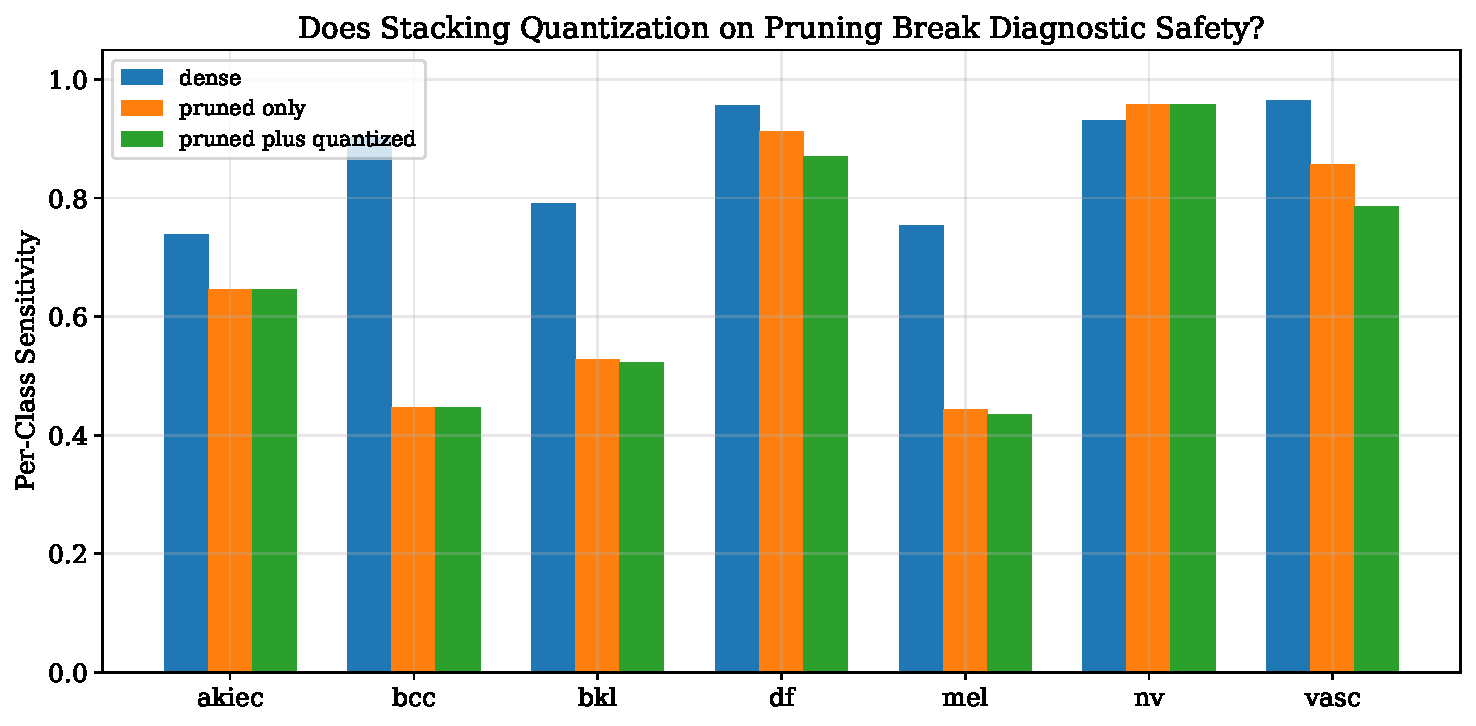
\includegraphics[width=0.95\textwidth]{../results/figures_local/fig5_stacking.pdf}
    \caption{Per-class sensitivity for dense, pruned, and pruned-plus-quantized models.}
    \label{fig:stacking}
\end{figure}

\subsection{Knowledge Distillation Before Pruning}
Distillation improves the dense Tiny model, but not its pruning robustness. As shown in Table~\ref{tab:kd}, the distilled Tiny model reaches balanced accuracy $0.861$, exceeding the directly fine-tuned Tiny baseline at $0.840$. However, after Wanda pruning at 50\% sparsity, the directly fine-tuned Tiny model remains better than the distilled Tiny model. Direct Tiny retains balanced accuracy $0.614$ and melanoma sensitivity $0.556$, while distilled Tiny falls to balanced accuracy $0.541$ and melanoma sensitivity $0.413$.

The ImageNet-only control performs poorly both before and after pruning, confirming that HAM10000 fine-tuning is essential. Overall, distillation helps dense performance but does not create pruning-robust features under the Wanda setup used here.

\begin{table}[H]
    \centering
    \caption{Knowledge distillation pre-treatment results on DeiT-Tiny.}
    \label{tab:kd}
    \begin{tabular}{llSS}
        \toprule
        Variant & Pruned & {Balanced Acc.} & {Mel. Sens.} \\
        \midrule
        Direct fine-tune & No  & 0.840 & 0.758 \\
        Direct fine-tune & Yes & 0.614 & 0.556 \\
        Distilled & No  & 0.861 & 0.744 \\
        Distilled & Yes & 0.541 & 0.413 \\
        ImageNet only & No  & 0.174 & 0.049 \\
        ImageNet only & Yes & 0.148 & 0.045 \\
        \bottomrule
    \end{tabular}
\end{table}

\begin{figure}[H]
    \centering
    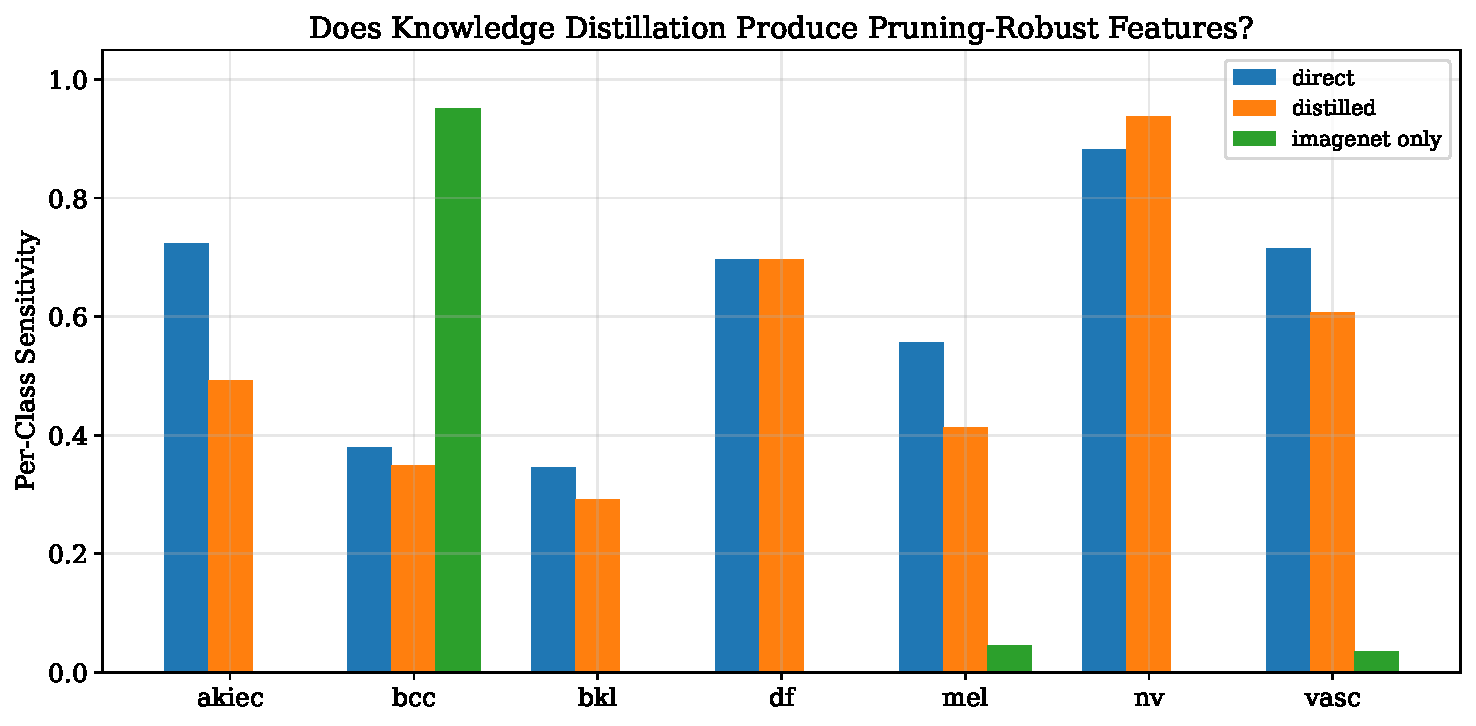
\includegraphics[width=0.95\textwidth]{../results/figures_local/fig6_kd_pretreatment.pdf}
    \caption{Per-class sensitivity after Wanda pruning for direct fine-tuning, distillation, and ImageNet-only initialization.}
    \label{fig:kd}
\end{figure}

\section{Discussion}
The central question of the project was whether activation-aware pruning protects diagnostic safety better than simple pruning baselines when compressing medical Vision Transformers. In our experiments, the answer is no. Wanda underperformed magnitude pruning on both DeiT-Tiny and DeiT-Small across the clinically important 50\% sparsity point. On DeiT-Small, the gap is particularly large: balanced accuracy falls from $0.813$ under magnitude to $0.685$ under Wanda, and melanoma sensitivity falls from $0.637$ to $0.444$.

This does not mean activation-aware pruning is inherently unhelpful in medical vision. The non-uniform sparsity experiment shows the opposite: once layer sensitivity is used to control where sparsity is assigned, Wanda recovers dramatically. This implies that Wanda's raw scores may not be enough on their own in this domain, but the combination of activation awareness and layer-level protection is promising. The failure mode appears to be poor sparsity placement rather than a total absence of useful information in activations.

Taylor pruning is another notable result. It consistently performs well and achieves the highest melanoma sensitivity at 50\% sparsity on DeiT-Small. This suggests that first-order loss sensitivity is a strong signal for clinically important features, even though the method is conceptually simpler than more elaborate post-hoc pruning pipelines.

Quantization is the safest and most deployment-friendly method in our experiments. The dense quantized model keeps essentially the same balanced accuracy while cutting model size by almost 4$\times$ and improving latency substantially. For systems where storage and CPU efficiency matter most, quantization appears to be a low-risk optimization. By contrast, the main danger lies in careless pruning.

The distillation result is mixed but informative. Distillation improves dense Tiny performance but does not help the student survive Wanda pruning better. This suggests that better dense features do not automatically translate into better sparse features. For future work, it may be necessary to couple distillation with sparsity-aware training or recovery fine-tuning rather than treating it only as a pre-treatment.

\section{Limitations}
Several limitations should be acknowledged.

First, this study uses only one medical dataset and one family of transformer backbones, so the conclusions may not generalize directly to other medical modalities or model architectures. Second, the experiments were run locally on an RTX 3060 Ti rather than on the originally planned A100 cluster environment. This affected runtime and practical batch-size choices, though not the overall experimental design.

Third, patch embedding was excluded from default pruning, which means the patch-embedding rows in the per-layer breakdown act as a control rather than a genuine pruned condition. This choice was intentional to avoid disproportionate degradation, but it should be stated clearly in the report. Fourth, the non-uniform allocation policy is simple: it uses ranked bins and fixed target sparsities. More sophisticated allocation strategies may perform better.

Finally, we focus on one-shot pruning without post-pruning recovery fine-tuning. Recovery training could change the ranking between criteria, especially at high sparsity.

\section{Conclusion}
This project investigated whether compressing medical Vision Transformers causes them to forget dangerous diseases first. Using HAM10000 and two DeiT backbones, we compared four pruning criteria and then studied non-uniform sparsity allocation, quantization stacking, and knowledge distillation.

Three clear conclusions emerged. First, activation-aware Wanda did not preserve melanoma sensitivity better than magnitude or Taylor pruning in this setting. Second, sensitivity-guided non-uniform sparsity allocation was the strongest rescue mechanism, substantially improving Wanda while keeping the same average sparsity. Third, INT8 quantization was largely safe and effective, both as a standalone compression method and as a final-stage addition after pruning. Distillation improved the dense Tiny baseline but did not improve pruning robustness.

Overall, the project reinforces a clinically important lesson: compression in medical AI should not be evaluated only by overall accuracy. Class-wise sensitivity, especially for rare and dangerous classes, can tell a very different story. In this study, pruning strategy and sparsity placement mattered much more than model size alone, and the safest practical deployment path appears to be careful pruning combined with quantization rather than aggressive activation-aware pruning without layer sensitivity control.

\section*{Reproducibility Note}
All experiments, checkpoints, masks, CSV logs, and report figures were generated from the local project codebase. The final result logs are stored under \texttt{results/logs\_local/}, and the final figures used in this report are stored under \texttt{results/figures\_local/}. This report was generated to match those final artifacts.

\bibliographystyle{plain}
\bibliography{references}

\end{document}
